\section{Results and Discussion} \label{sec:results}

In this section, we report annotate-and-reconstruct experiments comparing phylogeny reconstruction quality obtained across possible hereditary stratigraphy approaches.
These experiments seek to establish a holistic, evidence-driven synopsis of each approach's suitability across experimental use cases.
The following section, ``A Practicioner's Guide to Hereditary Stratigraphy,'' then synthesizes findings to suggest guidelines for selecting appropriate methods to apply in practice.

This section delves into three primary aspects of hereditary stratigraphy methodology:
\begin{enumerate}
\item surface- versus column-based implementation,
\item tilted versus steady (versus hybrid) retention, and
\item bit- versus byte-sized differentiae.
\end{enumerate}

In a final set of experiments, we investigate how reconstruction quality fares with increasing phylogeny scale.
Scale-up of subsampled tip count and of underlying population size are both considered.
This question is crucial to application of hereditary stratigraphy for very large simulation use cases --- in assessing the extent, if at all, annotation size would need to be boosted with increased experimental scale.

\subsection{Surface vs. Column Implementaiton} \label{sec:surface-vs-column}

\begin{figure*}
  \centering
  \begin{subfigure}[b]{0.5\textwidth}
    \centering
    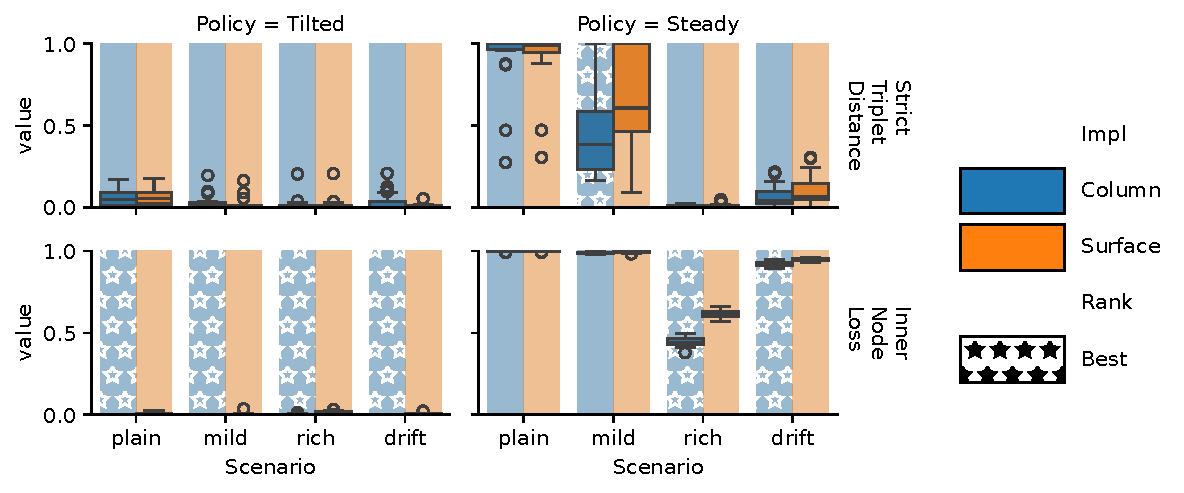
\includegraphics[width=\textwidth]{binder/binder/surf-vs-col/teeplots/annotation-size-bits=64+col=policy+differentia-width-bits=1+downsample=500+hue=impl+num-generations=100000+population-size=65536+post=teed-figure-subplots-adjust-right-0-72-teed-set-titles-row-templat.../e-row-name+row=variable+score=value+viz=peckplot+x=scenario+x-group=outer+y=value+ext=}
    \caption{Example reconstruction quality measure distributions. Lower is better.}
    \label{fig:col-vs-surf-example}
  \end{subfigure}%
  \begin{subfigure}[b]{0.5\textwidth}
    \centering
    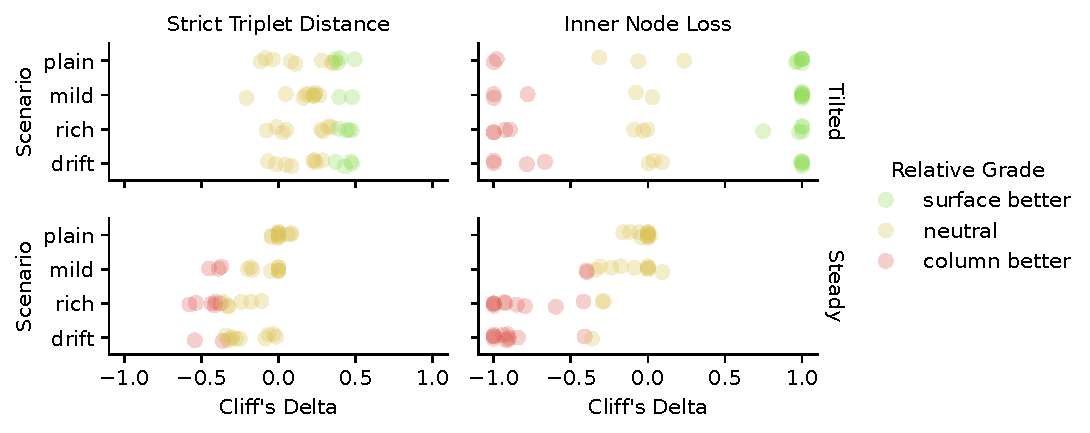
\includegraphics[width=\textwidth]{binder/binder/surf-vs-col/teeplots/col=metric+hue=relative-grade+kind=strip+post=teed-set-titles-col-template-col-name-row-template-row-name+row=policy+viz=catplot+x=cliff-s-delta+y=scenario+ext=}
    \caption{Reconstruction quality comparison outcomes.}
  \label{fig:col-vs-surf-overview}
  \end{subfigure}
  \caption{%
    \textbf{Does column- or surface-based instrumentation give higher-quality reconstruction?}
    Subpanel \ref{fig:col-vs-surf-overview} shows effect sizes of column-vs-surface comparisons for triplet distance and inner node loss metrics.
    Color coding indicates a significant outcome (Mann-Whitney U).
    Surface tends to outperform column under tilted policy and vice versa under steady policy.
    Subpanel \ref{fig:col-vs-surf-example} shows reconstruction quality effects for 64-bit size, bit-differentia annotations wit population size 65,536, downsample size 500, and 100k generations.
    Background hatching indicates significant outcome.
  }
  \label{fig:col-vs-surf-summary}
\end{figure*}


Recall that surface- and column-based annotation implementations differ in how differentia are organized within a hereditary stratigraphy annotation.
Surface-based implementation takes a lower-level approach that simplifies accessioning of new differentia and ensures full use of available memory space but sacrifices some control over the precise temporal distribution of retained differentiae.
Both implementations support tilted and steady retention policies.

Figure \ref{fig:col-vs-surf-summary} compares reconstruction quality for surface algorithms against their corresponding column implementation.
Outcomes differ notably between tilted and steady retention.

Under tilted retention, triplet distance (a measure of reconstruction accuracy) is equivalent or improved (in 14 / 48 scenarios) with surface-based implementation.
Inner node loss (a measure of reconstruction precision) improves in some scenarios and worsens in others.
Notably, shown in Supplementary Figure \ref{fig:col-vs-surf}, inner node loss improvement is seen in all treatments with byte-width differentiae, which are mechanistically more prone to create artifactual unresolved polytomies that drive inner node loss.
In sum, reconstruction quality of surface-based tilted retention can be considered equivalent or superior across the board to that of column-based implementation.

In contrast, under steady retention, surface-based implementation achieves worse triplet distance reconstruction in 11 / 48 scenarios and better triplet distance in no scenario.
Similarly, inner node loss is worse in 23 / 48 scenarios, including 4 / 12 byte-differentiae scenarios, and better in no scenario.
So, reconstruction quality of surface-based steady retention is equivalent or inferior to column-based implementation.

Why does the surface-based approach benefit reconstruction under one retention policy but not the other?
Compared to column-implementation, surface-implementation allows the tilted algorithm to retain more differentia within available annotation space.
Whereas the write-only design of the surface-based approach guarantees full use of buffer space, the column-based tilted retention holds space in reserve on account of discretization effects in tuning retention density.
In contrast, column-based steady retention makes full use of available space, giving the surface-based approach no advantage in this regard.
Although both approaches prune differentiae through comparable strided decimation procedures, the column implementation more systematically drops decimated differentiae from back to front.
This process ends up preserving more recent differentiae which, as we will see in the next set of experiments comparing steady and tilted retention, tends to benefit reconstruction quality.

Although surface-based implementation involves a trade-off between performance reconstruction quality in the steady case, it is notable that surface-based implementation provides uncompromised improvement in both runtime performance and data quality.

% We did this by using a simple simulation to generate phylogenies under different conditions with perfect tracking, then simulating heritage of hstrat annotations down the perfect tree and subsequent reconstruction.
% We could then compare the reconstruction that would have been obtained under approximate tracking to the underlying ground truth.

% To ensure generalizable results, we tested over a large number of evolutionary regimes, population sizes, instrumentation sizes, and instrumentation fingerprint sizes.

% We took three measures of reconstruction quality.
% The first measure, triplet distance, is a measure of accuracy --- it is the fraction of triplet tips that are correctly arranged in the reconstruction.
% Whereas this metric considers polytomies as distinct from separate branching events, our second measure is a lax variant of triplet distance that does not penalize penalties introduced into the reconstruction (i.e., due to uncertainty about branching order) or over-resolution of true polytomies into more nodes in the reconstruction.
% Finally, we also include inner node count, which provides a measure of the amount of precision achieved by reconstructions.
% Higher inner node count indicates that fewer branching events are being lumped together into polytomies due to insufficient information to differentiate them.
% This metric is only applicable to scenarios with fingerprint sizes larger than one bit (i.e., a byte), which are capable of generating non-bifurcating trees.

% The data tell two clear stories:
% \begin{enumerate}
% \item surface tilted algorithms create higher-quality reconstructions than column-based tilted algorithms and
% \item surface column algorithms create lower-quality reconstructions than column-based column algorithms.
% \end{enumerate}

\subsection{Steady vs. Tilted Retention} \label{sec:steady-vs-tilted}

\begin{figure*}
  \centering
  \begin{subfigure}[b]{0.42\textwidth}
    \centering
    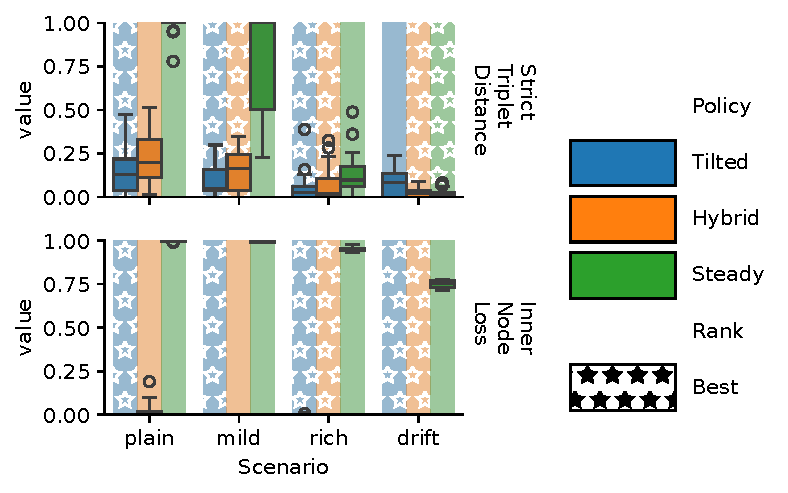
\includegraphics[width=\textwidth]{binder/binder/steady-vs-tilted/teeplots/annotation-size-bits=64+differentia-width-bits=1+downsample=500+hue=policy+num-generations=100000+population-size=65536+row=variable+score=value+viz=peckplot+x=scenario+x-group=outer+y=value+ext=}
    \caption{Example reconstruction quality distributions. Lower is better.}
    \label{fig:steady-vs-tilted-summary-example}
  \end{subfigure}%
  \begin{subfigure}[b]{0.58\textwidth}
    \centering
    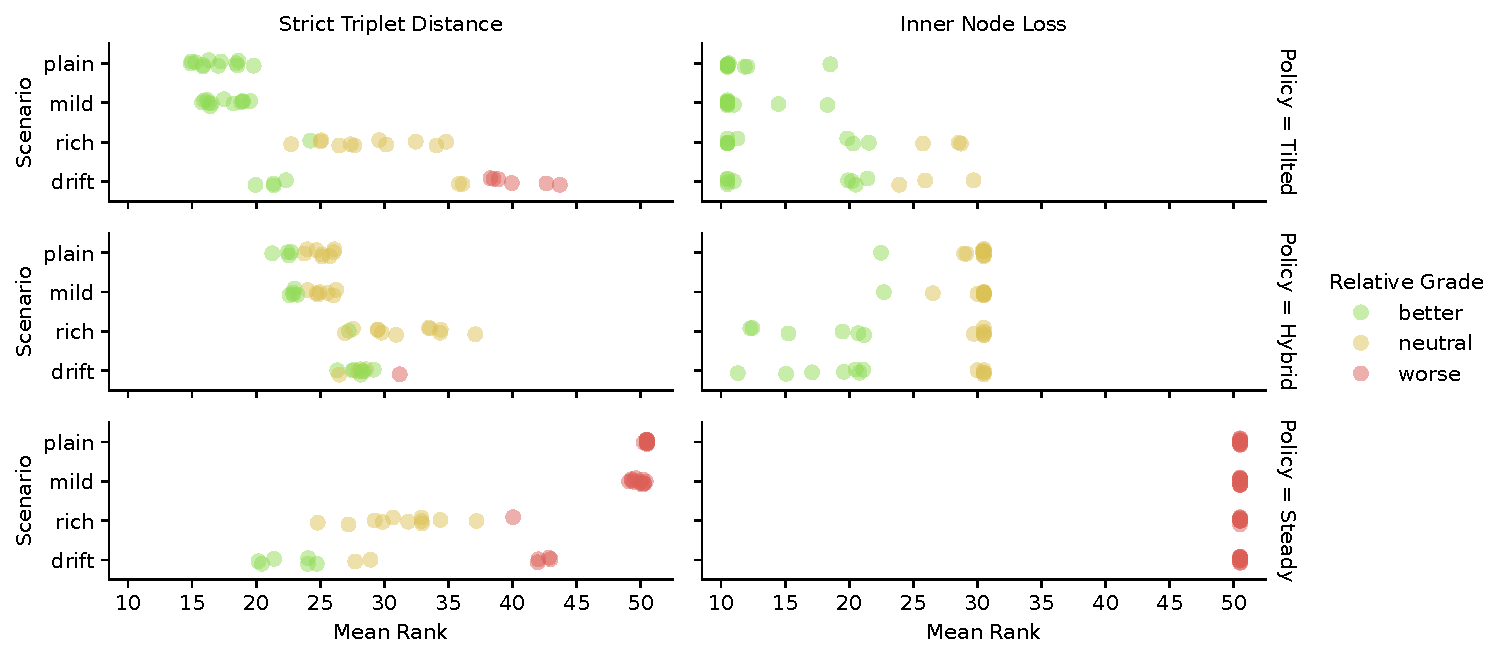
\includegraphics[width=\textwidth]{binder/binder/steady-vs-tilted/teeplots/col=metric+hue=relative-grade+kind=strip+row=policy+viz=catplot+x=mean-rank+y=scenario+ext=}
    \caption{Reconstruction quality comparison outcomes. Lower is better.}
    \label{fig:steady-vs-tilted-summary-overview}
  \end{subfigure}
  \caption{%
    \textbf{How does retention policy affect reconstruction quality?}
    \footnotesize
    Subpanel \ref{fig:steady-vs-tilted-summary-overview} shows mean rank among reconstruction error measures from tilted, hybrid, and steady retention policies across sensitivity analysis conditions.
    Each point represents an independent 20-replicate trial under different evolutionary conditions, instrumentation configuration (e.g., annotation size), and phylogenetic scale (e.g., reconstruction tip count).
    Color coding indicates significant outcome (Kruskal-Wallis H then Mann-Whitney U test).
    Lower is better.
    Tilted policy (top row) performs best in most evolutionary scenarios, except triplet distance under the highly phylogenetically-rich drift regime.
    Steady policy (bottom row) performs worst in most scenarios, except triplet distance under the drift regime.
    Hybrid policy performance has somewhat higher triplet distance reconstruction distance error in the plain and mild scenarios than tilted policy, but is robust to the drift regime.
    Subpanel \ref{fig:steady-vs-tilted-summary-example} shows reconstruction quality effects for 64-bit size, bit-differentia annotations with population size 65,536, downsample size 500, and 100k generations.
    Background hagching indicates significant outcome.
    See Supplementary Figure \ref{fig:steady-vs-tilted} for listing of reconstruction quality outcomes by sensitivity analysis condition \citep{moreno2024supplemental}.
  }
  \label{fig:steady-vs-tilted-summary}
\end{figure*}


Steady and tilted retention differ in the composition of differentia checkpoint records maintained within hereditary stratigraphy annotations.
Recall that steady policy spaces retained differentia evenly across history, while tilted policy retains more of more recent differentia.
The question of which policy gives higher quality reconstruction boils down to where precision in discerning the timing of branching events is most useful to resolving evolutionary history.
In the interest of even footing, we report results for each retention policy using its best-performing implementation, as established above: steady policy uses column implementation and tilted policy uses surface implementation.
We also consider a hybrid policy, which splits surface buffer space evenly between steady and tilted retention.

Figure \ref{fig:steady-vs-tilted-summary} overviews how reconstruction quality differs by retention policy across use case scenarios.
Across the board, steady policy yields phylogenetic reconstruction with heaviest inner node loss.
In contrast, tilted policy exhibits among the lowest inner node loss in all but six surveyed scenarios --- including all byte-differentia trials (Supplementary Figure \ref{fig:steady-vs-tilted}).
The hybrid policy has lower inner node loss in those six scenarios, which all involve evolutionary conditions with high phylogenetic richness.

Steady policy also consistently produces the worst triplet distance error in lower-phylogenetic-richness plain and mild structure evolutionary scenarios.
However, in scenarios with high phylogenetic richness, triplet distance error under steady retention fares better.
With rich ecological/spatial structure, triplet distance reconstruction error is largely indistinguishable among retention policies.
Further, steady policy triplet error actually significantly outperforms tilted policy in several instances under drift conditions.
In nearly all of these instances, though, hybrid policy triplet error performs comparably to steady retention.
In low phylogenetic richness plain and mild-structure scenarios, hybrid triplet error is comparable to tilted error in 9 / 24 scenarios and outperformed by tilted policy in 15 / 24 scenarios.

Across the inner node loss and triplet error quality measures, tilted retention frequently performs best and steady retention frequently performs worst.
However, tilted retention has worse triplet error in some scenarios with high phylogenetic richness.
Hybrid retention performs more consistently across evolutionary scenarios.
It exhibits consistently intermediate levels of inner node loss that, in absolute terms, tend not to be far off from tilted retention.
Triplet error for hybrid retention is often comparable to the better-performing of steady and tilted retention, or at least intermediate between them.
For greater detail of steady vs. tilted reconstruction quality outcomes broken down by treatment condition, see Supplementary Figure \ref{fig:col-vs-surf}.

\begin{figure*}
  \centering
    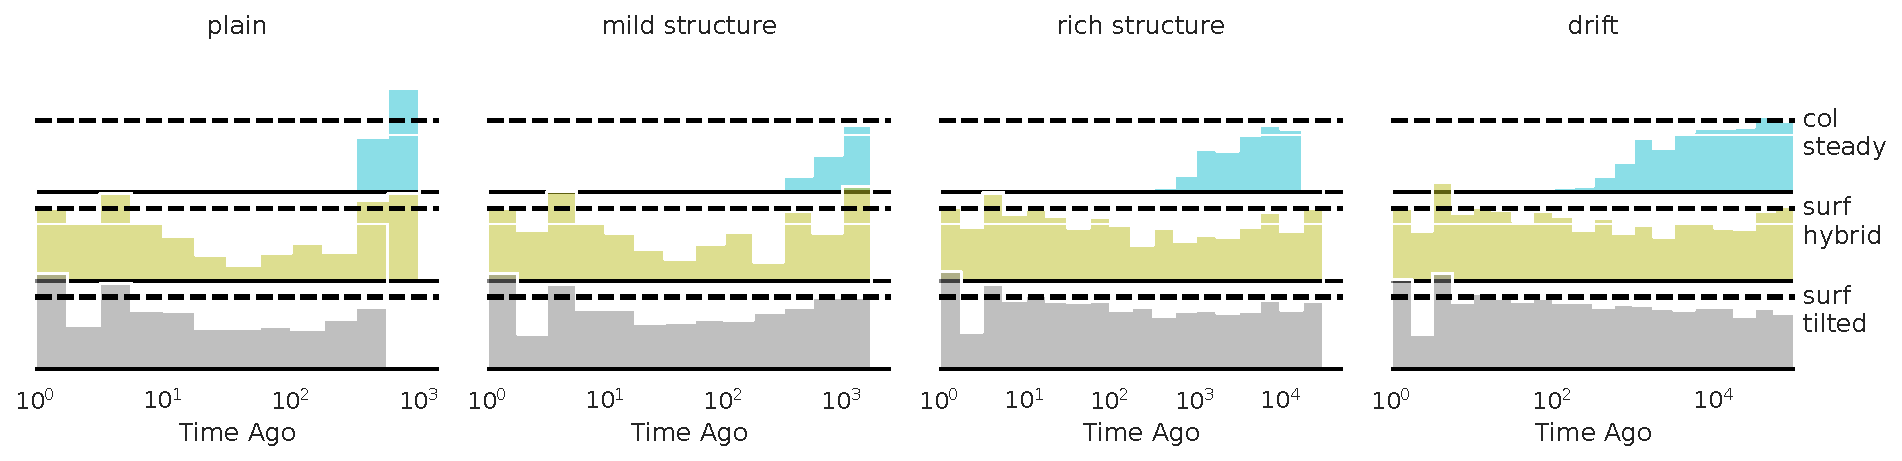
\includegraphics[width=\linewidth]{binder/binder/teeplots/annotation-size-bits=256+col=scenario+differentia-width-bits=8+hue=kind+row=algo+scale=npop65536-ngen100000+viz=joyhist+x=time-ago+ext=}
\caption{%
  \textbf{How does phylogeny structure differ by retention policy?}
  reconstruction node densities; 256-bit size, byte differentia
  TODO
}
  \label{fig:recency-structure}

\end{figure*}


Differences in retention of recent differentia explain the substantial advantage of tilted policy in use cases with low phylogenetic richness.
In such scenarios, frequent selective sweeps concentrate phylogenetic history over very recent history, meaning that lineage-branching events giving rise to a contemporary extant population occurred over a relatively short period of time.
Discerning these events, therefore, requires densely packed differentia checkpoints over recent history.
Otherwise, in the worst case, taxa would jump from all sharing the same lineage marker at one checkpoint to all having distinct checkpoint markers --- resulting in a catastrophic unresolved polytomy.
Steady retention maintains a uniform gap size between retained differentiae that grows linearly with generations elapsed, meaning that very recent history is sparsely covered, if at all.
The consequences of this deficiency can be seen in Figure \ref{fig:recency-structure}, which compares the density of reconstructed nodes to ground truth.
Reconstructions from steady policy are entirely missing branching events over the prefatory hundred or so generations.
Figures \labelcref{fig:bit-vs-byte-summary-byte-outcomes,fig:bit-vs-byte-summary-bit-outcomes} show reconstruction outcomes resulting under this inner node loss.
Under steady policy, very high levels of unresolved reconstruction occur in scenarios with low phylogenetic richness, particularly for recent branching events.
Example reconstructions exhibiting catastrophic comb polytomies characteristic of steady reconstruction of low-richness phylogenies can be seen in \ref{fig:examplepanel}.

% \subsection{Bit vs. Byte Differentia Width} \label{sec:bit-vs-byte}

% \begin{figure*}
  \centering

\begin{minipage}{\textwidth}
\begin{subfigure}[b]{0.4\textwidth}
\centering
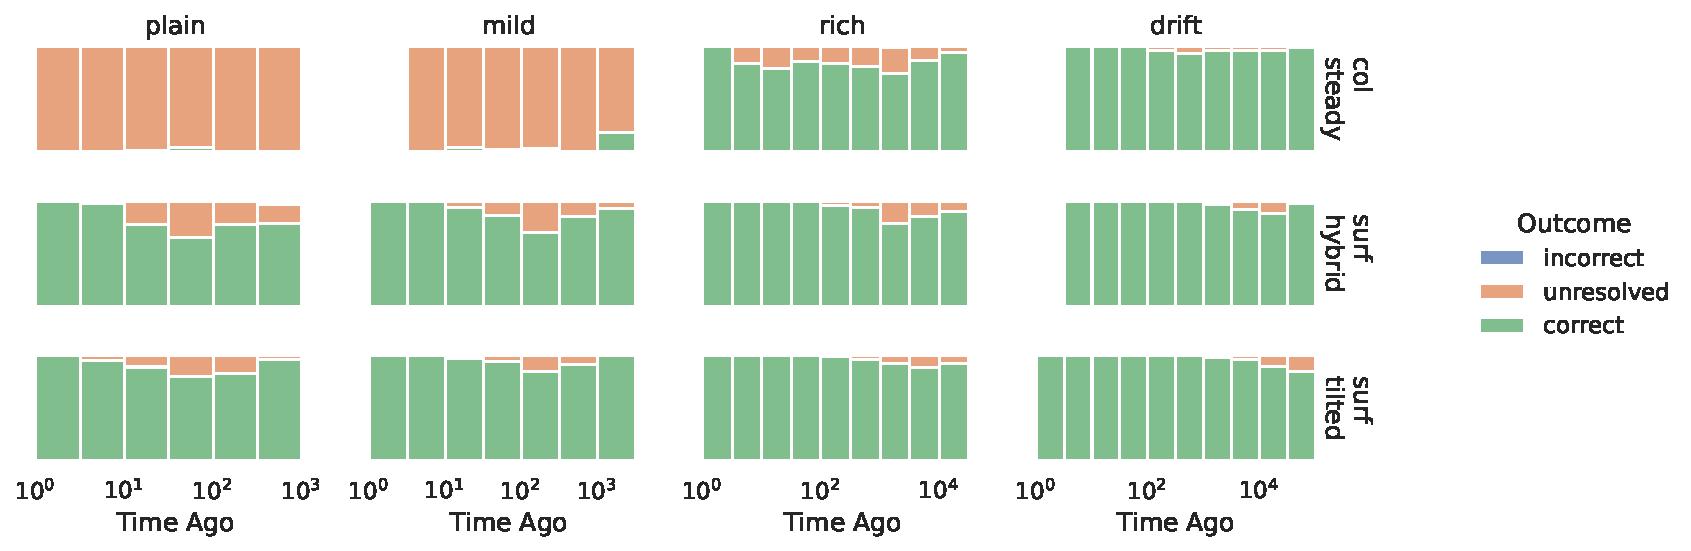
\includegraphics[height=1.2in,trim={0 0 5cm 0},clip]{binder/binder/teeplots/annotation-size=256+col=scenario+differentia-width=8+hue=outcome+kind=hist+multiple=fill+row=algo+scale=npop65536-ngen100000+viz=displot+x=time-ago+ext=}
\footnotesize
\caption{byte differentia outcomes; 256-bit annotation}
  \label{fig:bit-vs-byte-summary-byte-outcomes}
  \end{subfigure}%
\begin{subfigure}[b]{0.6\textwidth}
\centering
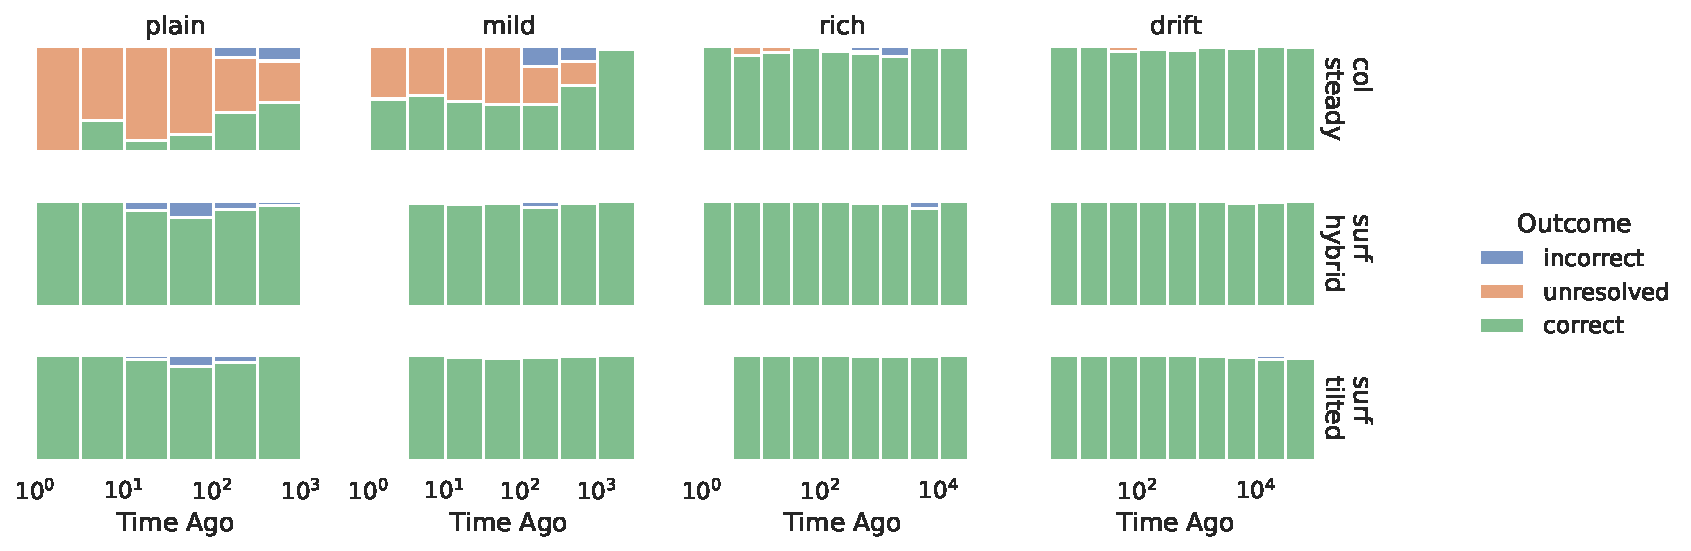
\includegraphics[height=1.2in]{binder/binder/teeplots/annotation-size=256+col=scenario+differentia-width=1+hue=outcome+kind=hist+multiple=fill+row=algo+scale=npop65536-ngen100000+viz=displot+x=time-ago+ext=}
\footnotesize
\caption{bit differentia outcomes; 256-bit annotation}
\label{fig:bit-vs-byte-summary-bit-outcomes}
\end{subfigure}
% \begin{subfigure}[b]{0.6\textwidth}
% \centering
% 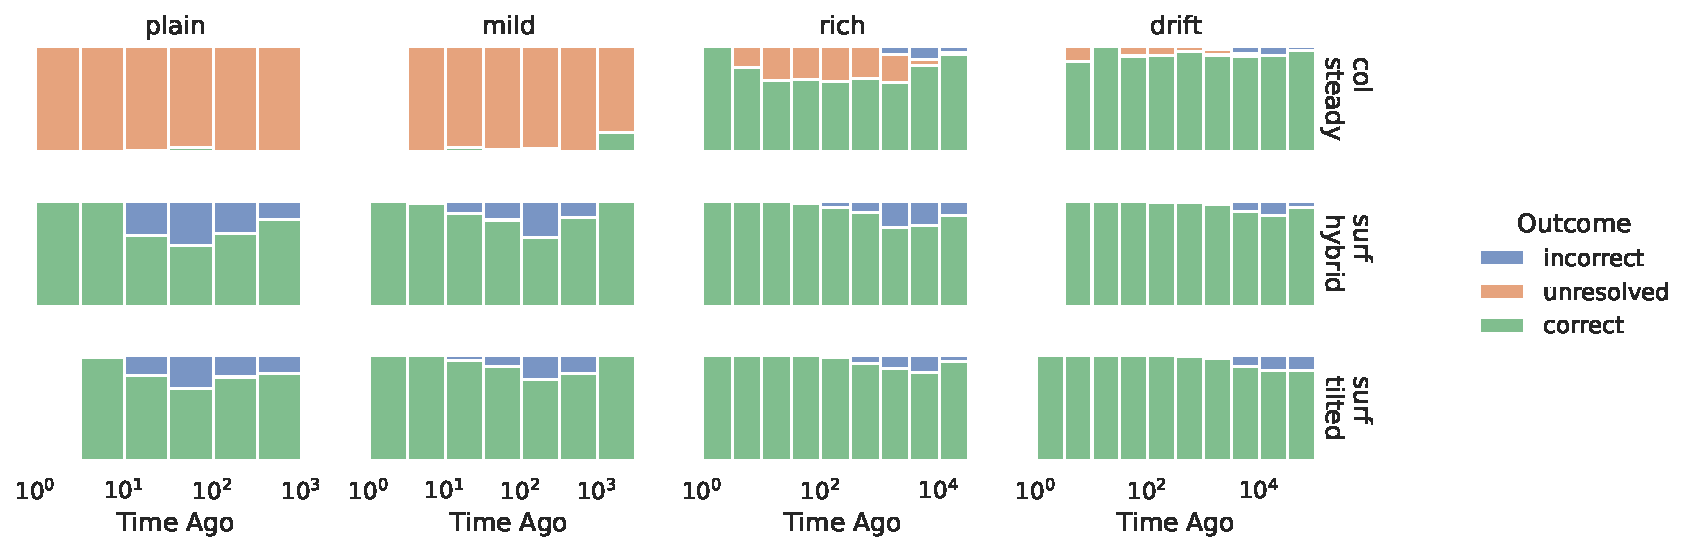
\includegraphics[height=1.2in]{binder/binder/teeplots/annotation-size=32+col=scenario+differentia-width=1+hue=outcome+kind=hist+multiple=fill+row=algo+scale=npop65536-ngen100000+viz=displot+x=time-ago+ext=}
% \caption{32-bit annotation, bit differentia}
% \end{subfigure}
\end{minipage}
% \begin{subfigure}[b]{0.4\textwidth}
%   \centering
%   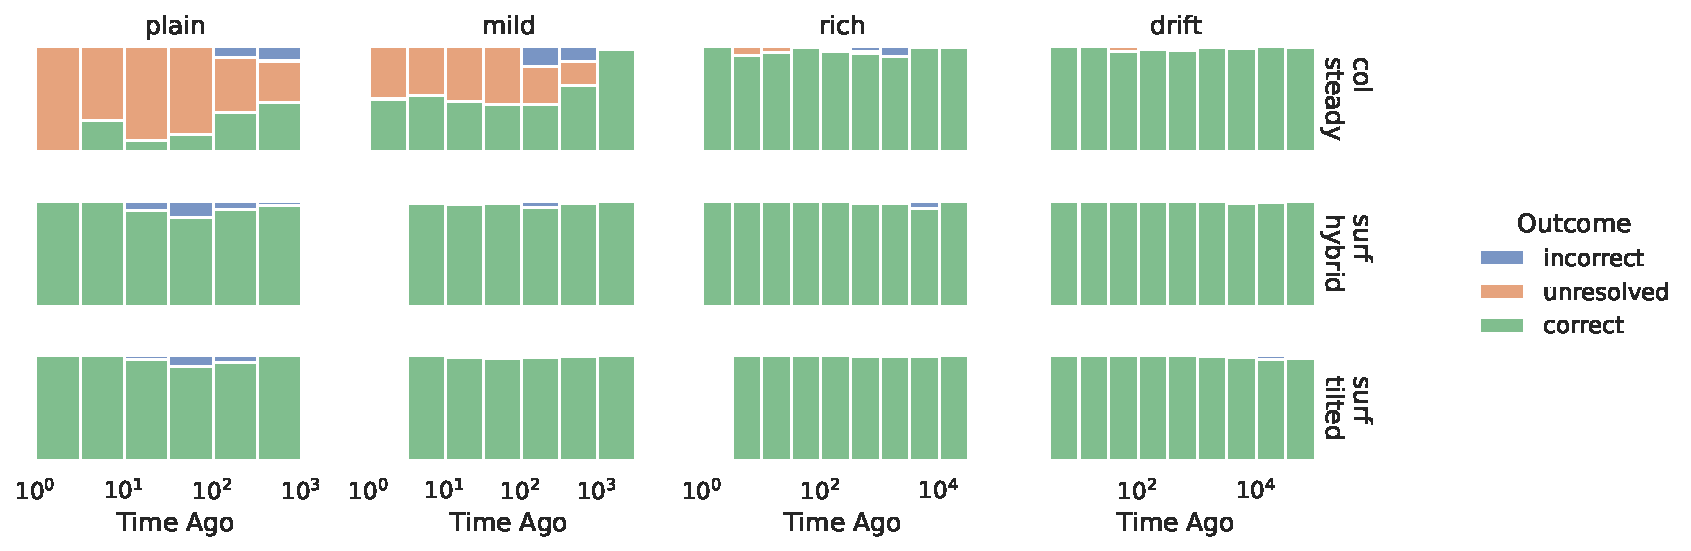
\includegraphics[height=1.2in,trim={0 0 5cm 0},clip]{binder/binder/teeplots/annotation-size=256+col=scenario+differentia-width=1+hue=outcome+kind=hist+multiple=fill+row=algo+scale=npop65536-ngen100000+viz=displot+x=time-ago+ext=}
%   \caption{reconstruction outcomes; 256-bit annotation, bit differentia}
%   \end{subfigure}%
  \begin{subfigure}[b]{\textwidth}
    \centering
    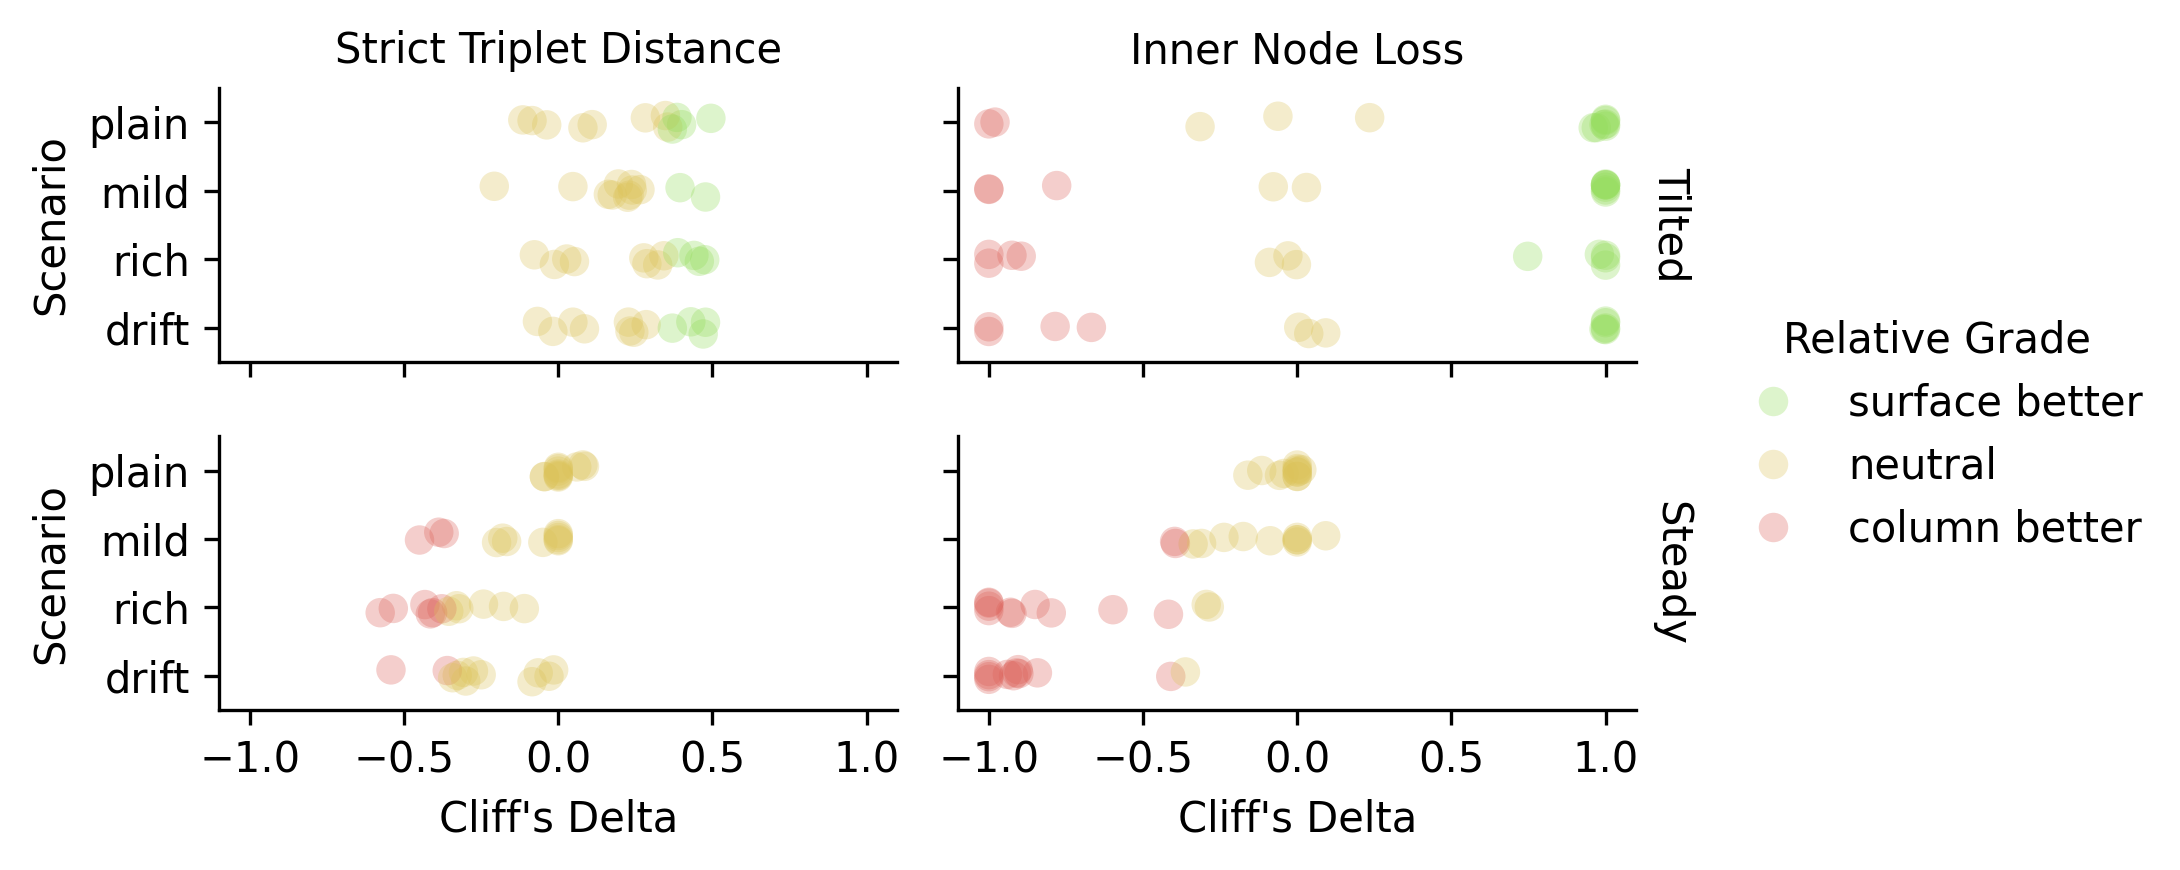
\includegraphics[width=0.8\linewidth]{binder/binder/bit-vs-byte/teeplots/col=metric+hue=relative-grade+kind=strip+row=policy+viz=catplot+x=cliff-s-delta+y=scenario+ext=}
    \footnotesize
    \caption{Reconstruction quality of byte differentia, relative to bit differentia; 256-bit size annotation}
  \label{fig:bit-vs-byte-summary-quality}
  \end{subfigure}%
\caption{%
  \textbf{How does differentia width affect reconstruction quality?}
  \footnotesize
   Top panels show reconstruction outcomes for phylogenetic branching events (Figure \ref{fig:hstrat-failure-modes}) under bit- and byte-width differentiae, respectively.
   Outcomes are binned by time ago (ranging from most recent to most ancient).
   Bottom panel compares reconstruction quality metrics between reconstructions from annotations with bit- and byte-width differentiae.
   Color coding indicates significance, with red indicating better bit-width differentia performance and green indicating better byte-width differentia performance.
   Byte-width differentiae consistently underperform bit-width differentia in inner node loss and strict triplet distance measures.
   However, byte-width differentiae outperform bit-width differentia in the lax triplet distance measure, which does not penalize polytomy triplets, i.e., isolating incorrect reconstruction from unresolved reconstruction (Figure \ref{fig:hstrat-failure-modes}).
  See Supplementary Figure \ref{fig:bit-vs-byte} for listing of effects by sensitivity analysis condition \citep{moreno2024supplemental}.
}
  \label{fig:bit-vs-byte-summary}

\end{figure*}


% We now turn to consider the role of differentia size in hereditary stratigraphy reconstruction quality.
% Intuitively, tuning differentia size would seem to trade-off between accuracy and precision.
% Larger differentiae reduce the probability of spurious collision, which falsely makes lineages appear more closely related than they actually are.
% Note, in particular, that reconstructions from bit-sized differentia estimate all history as bifurcating, because each checkpoint can only discern two distinct lineages.
% On the other hand, for fixed annotation size, widening differentia necessarily reduces differentia count.
% Thus, differentia size diminishes the granularity at which branching events can be dated.

% To ascertain the actual effects of differentia width on reconstruction quality, we performed annotate-and-reconstruct experiments across a variety of use case scenarios.
% These experiments used 256-bit-sized annotations, comprised of either 256-bit-sized differentiae or 32-byte-sized differentiae.
% Figure \ref{fig:bit-vs-byte-summary-quality} overviews the relative performance of bit- and byte-width differentiae on triplet distance and inner node loss quality measures.
% (Supplementary Figure \ref{fig:bit-vs-byte} presents these results in greater detail, showing reconstruction outcomes for each treatment condition surveyed.)
% However, byte-width differentia consistently produces reconstructions with lower inaccuracy --- as measured by lax triplet distance, which does not penalize unresolved reconstruction.
% Byte-width's lower incidence of incorrect reconstruction outcomes is apparent in Figures \labelcref{fig:bit-vs-byte-summary-byte-outcomes,fig:bit-vs-byte-summary-bit-outcomes}, which assess rates of correct, incorrect, and unresolved reconstruction outcomes across evolutionary history.
% Unlike bit-width annotations, byte-width methods produce almost no incorrect reconstruction outcomes.
% However, owing to unresolved byte-width outcomes, bit-width annotations nonetheless have a higher rate of correct outcomes.
% Figure \ref{fig:bit-vs-byte-summary-quality} indeed confirms that, in nearly all cases, bit-width differentiae produce more informative depictions of phylogenetic history, as measured by strict triplet distance.

% \subsection{Reconstruction Quality vs. Phylogeny Scale} \label{sec:scaling}
% % https://tex.stackexchange.com/a/159294/316176
\newcommand{\rulesep}{\unskip\ \vrule\ }

\begin{figure*}
  \centering
  \begin{subfigure}[b]{0.33\textwidth}
    \centering
    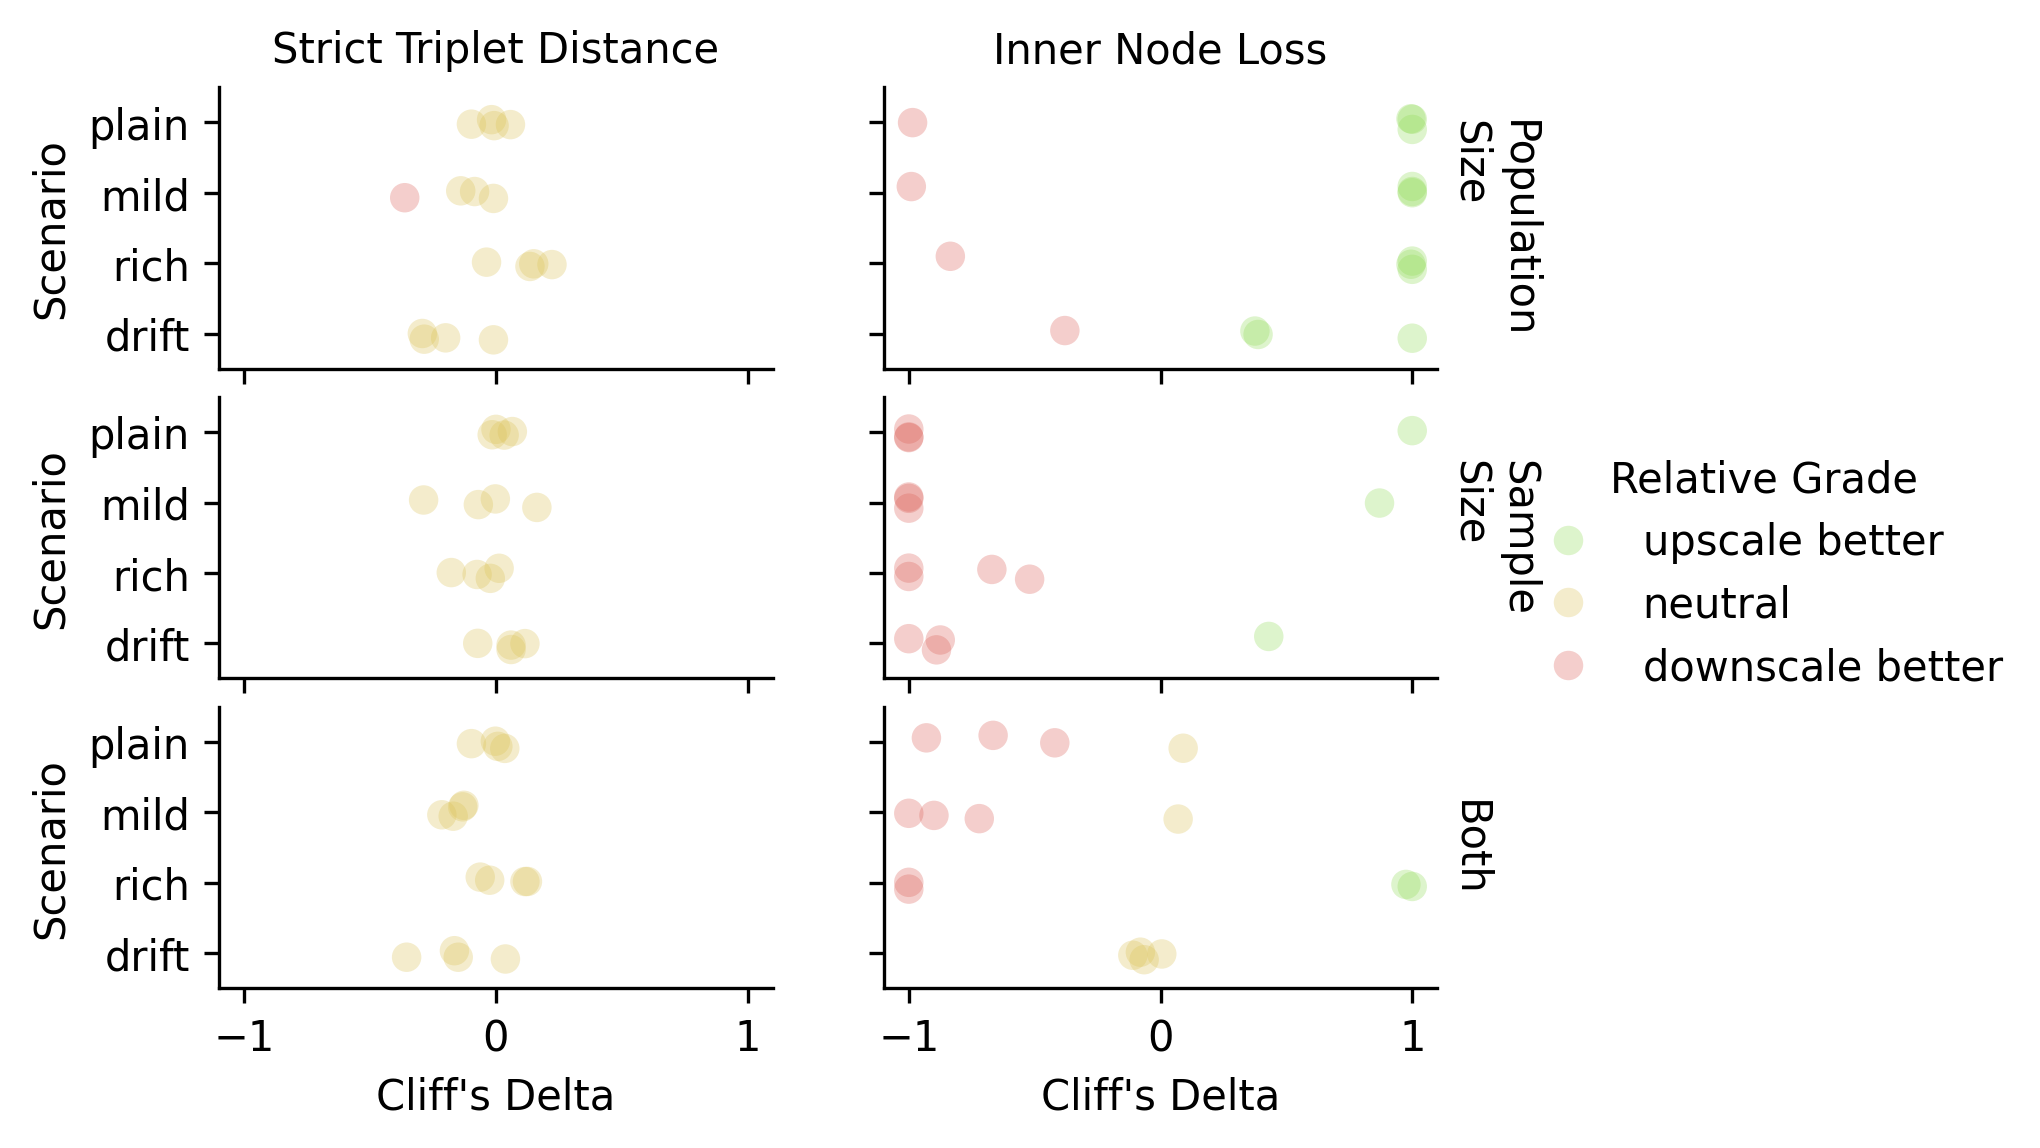
\includegraphics[height=1.7in,trim={0 0 5cm 0},clip]{binder/binder/dsamp-popsize-scale/teeplots/col=metric+hue=relative-grade+kind=strip+policy=tilted+row=scaling-factor+viz=catplot+x=cliff-s-delta+y=scenario+ext=}
    \caption{tilted retention policy (surface)}
  \end{subfigure}%
  \rulesep %
  \begin{subfigure}[b]{0.26\textwidth}
    \centering
    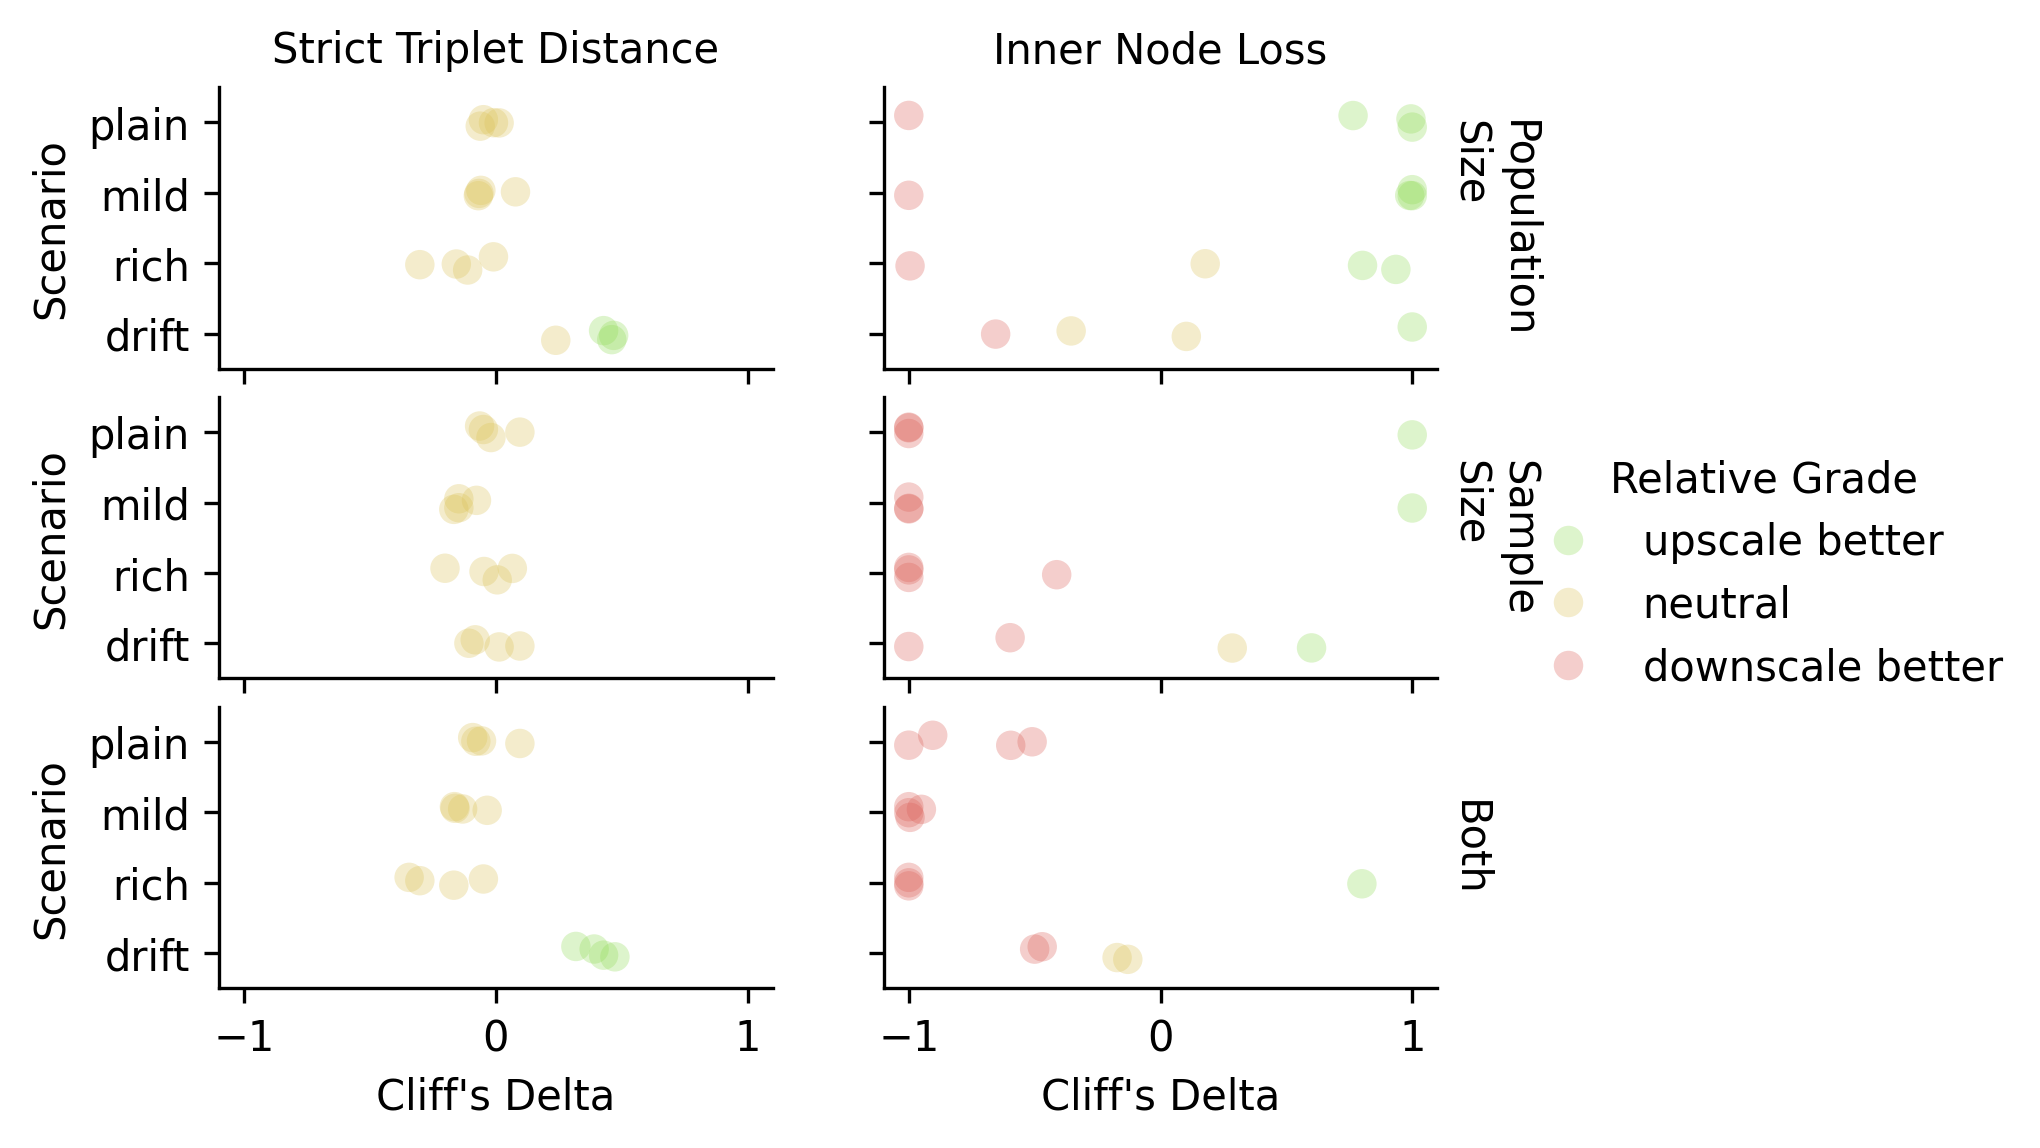
\includegraphics[height=1.7in,trim={2cm 0 5cm 0},clip]{binder/binder/dsamp-popsize-scale/teeplots/col=metric+hue=relative-grade+kind=strip+policy=hybrid+row=scaling-factor+viz=catplot+x=cliff-s-delta+y=scenario+ext=}
    \caption{hybrid retention policy (surface)}
  \end{subfigure}%
  \rulesep %
  \begin{subfigure}[b]{0.39\textwidth}
    \centering
    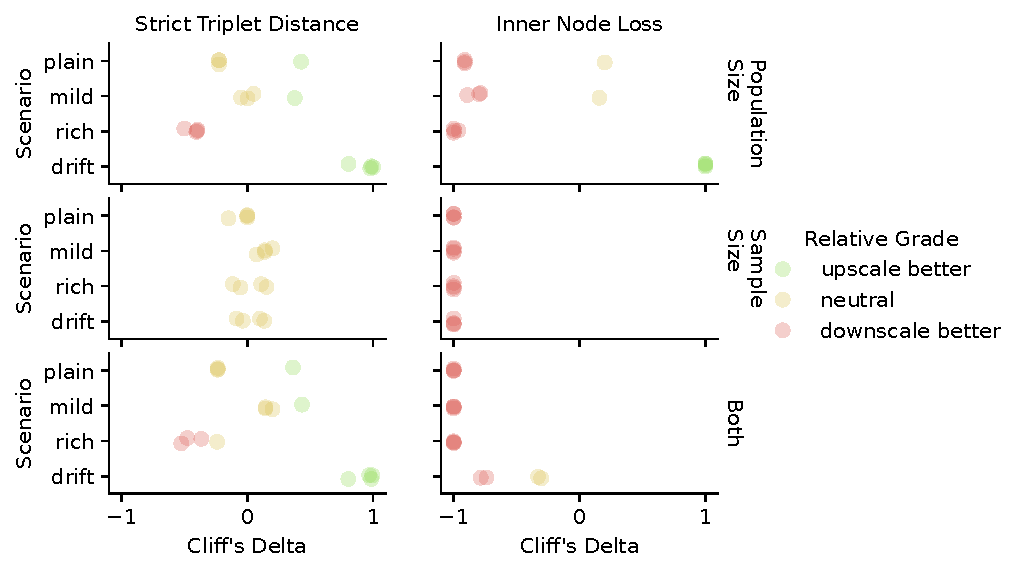
\includegraphics[height=1.7in,trim={2cm 0 0 0},clip]{binder/binder/dsamp-popsize-scale/teeplots/col=metric+hue=relative-grade+kind=strip+policy=steady+row=scaling-factor+viz=catplot+x=cliff-s-delta+y=scenario+ext=}
    \caption{steady retention policy (column)}
  \end{subfigure}
  \caption{%
  \textbf{How does scale impact reconstruction quality?}
  \footnotesize
  Each dot is a Cliff's Delta effect size of downscale-vs-upscale comparison under one sensitivity analysis condition.
  Color coding indicates a significant outcome (Mann-Whitney U).
  In order, rows show scaling outcomes for increasing population size, population subsample size (i.e., tree tip count), and both these factors.
  For tilted and hybrid policies, scaling had minimal effects on triplet distance and no systematic effect on inner node loss.
  Inner node loss worsened when scaling sample size, with and without scaling population size.
  Scaling effects were more variable under steady retention policy.
  See Supplementary Figures \labelcref{fig:dsamp-popsize-scale-hybrid,fig:dsamp-popsize-scale-steady,fig:dsamp-popsize-scale-tilted} for listing of effects by sensitivity analysis condition.
  }
  \label{fig:scaling-summary}
\end{figure*}

% The goal of hereditary stratigraphy methods is to empower new frontiers in digital evolution that harness parallel and distributed computing methods to realize scale-dependent experiments tackling phenomena like evolutionary transitions, eco-evolutionary dynamics, and open-endedness \citep{moreno2022exploring,dolson2021digital,channon2019maximum}.
% We also hope it will prove useful in future application-oriented work using massively parallel and distributed computing for evolutionary optimization.
% Given these objectives, the scaling behavior of hereditary stratigraphy is of key concern.
% Here, we consider two aspects of potential scale-up: (1) the number of taxa sampled for phylogenetic reconstruction and (2) the size of the underlying population.
% Experiments test how reconstruction quality fares with changes in scale along both fronts, across a variety of use case scenarios.
% Supplementary Figures \labelcref{fig:dsamp-popsize-scale-hybrid,fig:dsamp-popsize-scale-steady,fig:dsamp-popsize-scale-tilted} detail the use case scenarios surveyed and summarize reconstruction quality outcomes of phylogeny scale-up under each scenario.

% Scaling results for reconstruction accuracy, measured by triplet distance, are promising.
% Under tilted and hybrid policies, triplet distance error is robust across kinds of phylogenetic scaling --- population size, sample size, and both simultaneously.
% Reconstruction accuracy decreases significantly in only one case under the tilted policy.
% Results under the steady policy are more variable, with triplet distance worsening in 7 cases but improving in 11 cases.

% Inner node loss, under hybrid and tilted retention, is generally also robust to population scaling.
% For these policies, inner node loss worsens only in use cases with byte-width differentiae (Supplementary Figures \labelcref{fig:dsamp-popsize-scale-hybrid,fig:dsamp-popsize-scale-tilted}).
% In other cases, inner node loss actually often improves with population scale.
% Sample size scaling, however, tends to aggravate inner node loss --- whether in isolation or in concert with population size scaling.
% As an exception, we do not see inner node loss worsen with larger sample size in some cases with byte-width differentia under tilted and hybrid policies (Supplementary Figures \labelcref{fig:dsamp-popsize-scale-hybrid,fig:dsamp-popsize-scale-tilted}).
% Likewise, inner node loss remains stable for tilted retention under drift conditions (Supplementary Figure \labelcref{fig:dsamp-popsize-scale-tilted}).
